%
% design.tex
%
% Copyright (C) 2022 by SpaceLab.
%
% Camera Payload Preliminary Design Review
%
% This work is licensed under the Creative Commons Attribution-ShareAlike 4.0
% International License. To view a copy of this license,
% visit http://creativecommons.org/licenses/by-sa/4.0/.
%

%
% \brief Design slides.
%
% \author Gabriel Mariano Marcelino <gabriel.mm8@gmail.com>
% \author Vitória Beatriz Bianchin <vitoriabbianchin@gmail.com>
% \author Caique Sales de Miranda Gomes <kiqsmg@gmail.com>
%
% \version 0.1.0
%
% \date 2022/06/24
%


\begin{frame}{Specifications}

    \begin{itemize}
        \item \textbf{Sensor type}: RGB
        \item \textbf{Pixel size}: 2,2 $\times$ 2,2 $\mu$m
        \item \textbf{Max. Resolution}: 1600 $\times$ 1200 px
        \item \textbf{Field of View (FoV)}: \textcolor{red}{TBD}
        \item \textbf{Storage}: 16 MB (Flash NAND)
        \item \textbf{Power supply}: 3V3 @ \textcolor{red}{TBD} mA
        \item \textbf{Interfaces}:
            \begin{itemize}
                \item \textbf{Control/Data}: SPI and/or CAN
                \item \textbf{Debug}: UART
                \item \textbf{Programming}: JTAG
            \end{itemize}
    \end{itemize}

\end{frame}

% #########################################################################
% #########################################################################

\begin{frame}{Electrical Block Diagram}

    \begin{figure}[!ht]
        \begin{center}
            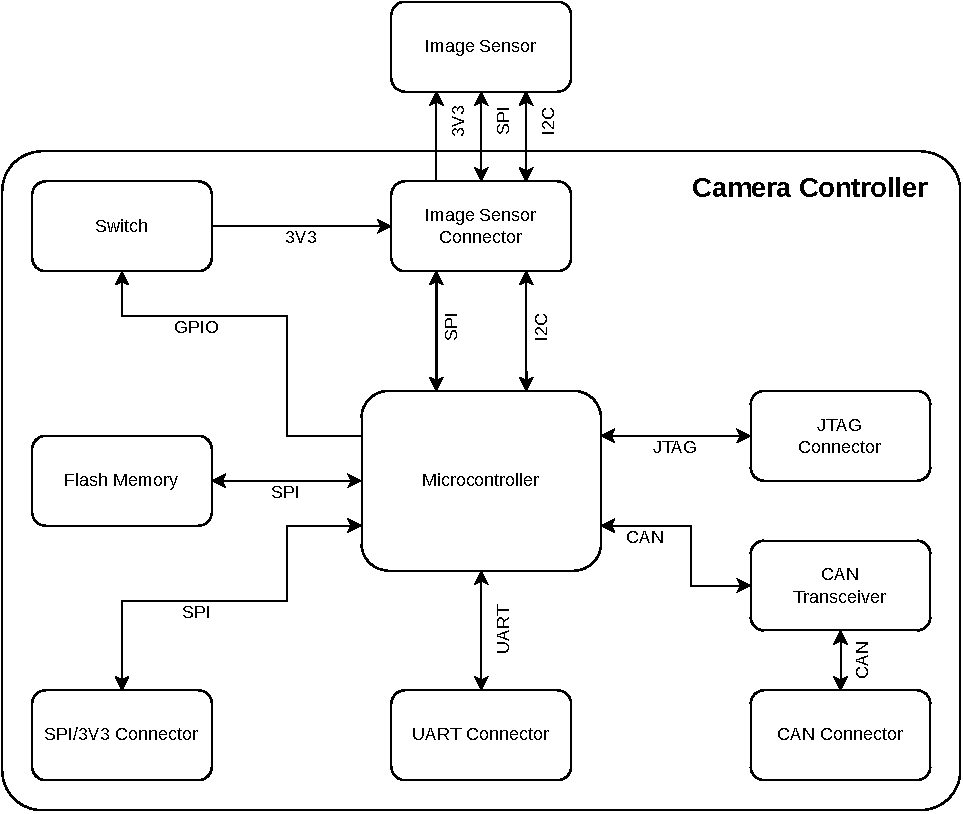
\includegraphics[scale=0.5]{figures/block-diagram}
        \end{center}
    \end{figure}

\end{frame}

% #########################################################################
% #########################################################################

\begin{frame}{Bill Of Materials}

    \begin{table}[!htb]\tiny
        \centering
        \label{tab:bom}
        \begin{tabular}{lL{2cm}cc}
            \toprule[1.5pt]
            \textbf{Component} & \textbf{Description} & \textbf{Partnumber} & \textbf{Quantity} \\
            \midrule
            Microcontroller        & ARM Cortex M3                & STM32F103C8T6        & 1 \\
            Flash Memory           & NOR 128 Mbit                 & W25Q128JVSIM TR      & 1 \\
            Switch                 & Load switch                  & TPS2010AD            & 1 \\
            CAN Transceiver        & CAN transceiver              & TCAN330GD            & 1 \\
            SPI/3V3 Connector      & PicoBlade 6 pin              & 532610671            & 1 \\
            UART Connector         & PicoBlade 3 pin              & 532610371            & 1 \\
            CAN Connector          & PicoBlade 3 pin              & 532610371            & 1 \\
            Image Sensor Connector & Female header 8 pin straight & -                    & 1 \\
            JTAG Connector         & Male header 4 pin angled     & -                    & 1 \\
            Image Sensor Module    & Arducam Mini 2MP Plus        & -                    & 1 \\
            Crystal                & 8 MHz crystal                & ECS-80-10-33-CHN-TR3 & 1 \\
            Lens                   & M12 lens                     & \textcolor{red}{TBD} & 1 \\
            Case                   & Aluminum case                & Custom               & 1 \\
            \bottomrule[1.5pt]
        \end{tabular}
    \end{table}

\end{frame}

% #########################################################################
% #########################################################################

\begin{frame}{Camera Sensor Module}

    \begin{columns}[t]
        \begin{column}[t]{0.6\textwidth}
            \begin{itemize}
                \item Module: \href{https://www.arducam.com/product/arducam-2mp-spi-camera-b0067-arduino/}{\textcolor{blue}{\underline{Arducam Mini 2MP Plus}}}
                \item Image sensor: OV2640
                \item Sensor type: RGB CMOS
                \item Res.: 2 MP (1600 $\times$ 1200 px)
                \item Power supply: 3,3/5 V
                \item Interfaces:
                    \begin{itemize}
                        \item Control: I$^{2}$C
                        \item Data: SPI
                    \end{itemize}
                \item Lens mount: M12
                \item Dimensions: 34 $\times$ 24 mm
            \end{itemize}
        \end{column}
        \begin{column}[t]{0.4\textwidth}
            \vspace{1cm}
            \begin{figure}[!ht]
                \begin{center}
                    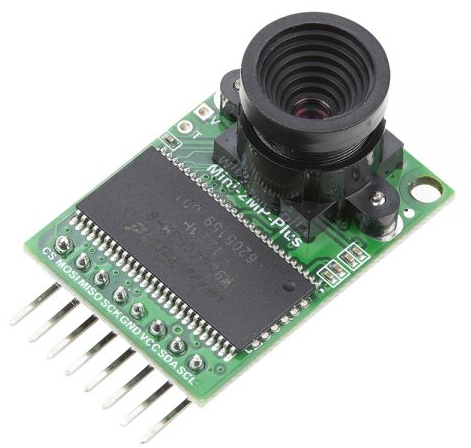
\includegraphics[width=4cm]{figures/arducam-2mp}
                \end{center}
            \end{figure}
        \end{column}
    \end{columns}

\end{frame}

% #########################################################################
% #########################################################################

\begin{frame}{Camera Sensor Module: Architecture}

    \begin{figure}[!ht]
        \begin{center}
            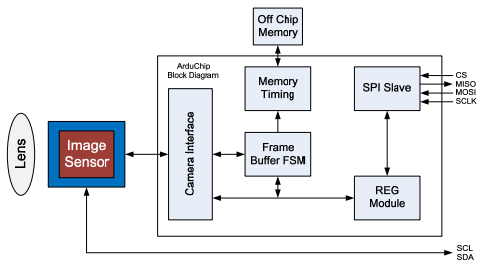
\includegraphics[width=8cm]{figures/arducam-block-diagram}
        \end{center}
    \end{figure}        
    
    \begin{itemize}
        \item ArduChip: FPGA (Lattice)
        \item Off Chip Memory: FIFO
        \item Image Sensor: OmniVision OV2640
    \end{itemize}
                        
\end{frame}             
 
% #########################################################################
% #########################################################################

\begin{frame}{Camera Sensor Module: Dimensions}

    \begin{figure}[!ht]
        \begin{center}
            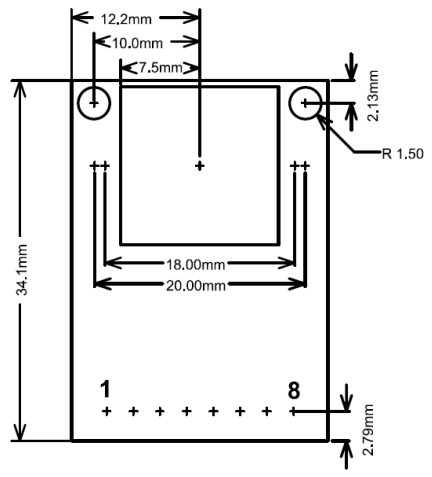
\includegraphics[width=6cm]{figures/arducam-dimensions}
        \end{center}
    \end{figure}        
    
\end{frame}             

% #########################################################################
% #########################################################################

\begin{frame}{Controller}

\textcolor{blue}{Colocar imagem do 3D da placa + resumo das specs. da placa}

\end{frame}

% #########################################################################
% #########################################################################

\begin{frame}{Optic System}

    \begin{itemize}
        \item Mount: M12
        \item FoV: XX$^{\circ}$ \textcolor{red}{TBD}
        \item With IR-filter
        \item Focus: Fixed, infinity
    \end{itemize}

\end{frame}

% #########################################################################
% #########################################################################

\begin{frame}{Mechanical Structure}

\textcolor{blue}{Colocar info e imagens do case de alumínio!!}

\end{frame}

% #########################################################################
% #########################################################################

\begin{frame}{Interface Requirements (ICD)}

\end{frame}

% #########################################################################
% #########################################################################

\begin{frame}{Power Consumption}

    \begin{itemize}
        \item ...
    \end{itemize}

\end{frame}

% #########################################################################
% #########################################################################

\begin{frame}{Dimensions}

    \textcolor{blue}{COLOCAR DESENHO COM DIMENSÕES!!!!}

\end{frame}

% #########################################################################
% #########################################################################

\begin{frame}{Satellite Integration: GOLDS-UFSC}

\textcolor{blue}{Colocar imagens da câmera instalada no GOLDS-UFSC (3D)}

\end{frame}

% #########################################################################
% #########################################################################

\begin{frame}{Firmware}

    \begin{itemize}
        \item OS: FreeRTOS
        \item ...
    \end{itemize}

\end{frame}

% #########################################################################
% #########################################################################

\begin{frame}{Firmware: Development Environment}

    \begin{columns}[t]
        \begin{column}[t]{0.6\textwidth}
            \begin{itemize}
                \vspace{0.4cm}
                \item Hardware: Generic STM32 Cortex-M3 dev kit
                \vspace{0.4cm}
                \item Programmer: ST-Link V2
                \vspace{0.4cm}
                \item Compiler: GCC (arm-none-eabi-XXX)
                \vspace{0.4cm}
                \item Programming tool: \href{https://github.com/stlink-org/stlink}{\textcolor{blue}{\underline{stlink}}}
            \end{itemize}
        \end{column}
        \begin{column}[t]{0.4\textwidth}
            \begin{figure}[!ht]
                \begin{center}
                    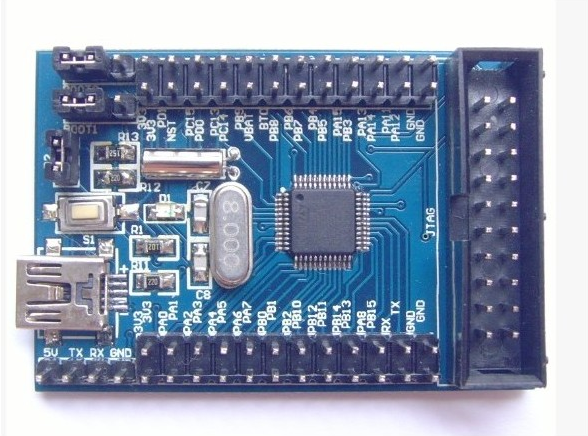
\includegraphics[width=4cm]{figures/stm32-dev-kit}
                \end{center}
            \end{figure}
            \begin{figure}[!ht]
                \begin{center}
                    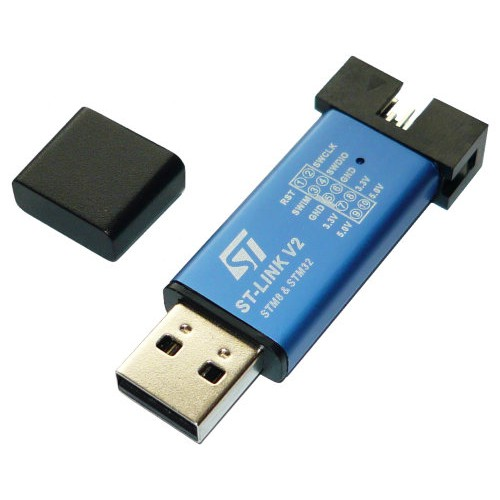
\includegraphics[width=3.5cm]{figures/stlink-v2}
                \end{center}
            \end{figure}
        \end{column}
    \end{columns}
\end{frame}

% #########################################################################
% #########################################################################

\begin{frame}{Firmware: Commands}

\begin{table}[!htb]
    \centering
    \label{tab:commands}
    \begin{tabular}{cll}
        \toprule[1.5pt]
        \textbf{ID} & \textbf{Command} & \textbf{Parameters}\\
        \midrule
        1 & Read ID                 & None \\
        2 & Power On/Off sensor     & 1 or 0 \\
        3 & Take picture            & None \\
        4 & Enable periodic capture & None \\
        5 & Read last picture       & None \\
        6 & Delete last picture     & None \\
        7 & Erase memory            & None \\
        8 & Set parameter           & Parameter ID + Parameter value \\
        9 & Get parameter           & Parameter ID \\
        \bottomrule[1.5pt]
    \end{tabular}
\end{table}

\end{frame}

\begin{frame}{Firmware: Commands}

\begin{table}[!htb]
    \centering
    \label{tab:parameters}
    \begin{tabular}{clll}
        \toprule[1.5pt]
        \textbf{ID} & \textbf{Name} & \textbf{Type} & \textbf{Access} \\
        \midrule
        0 & Module ID                   & uint16 & R\\
        1 & Sensor status               & uint8  & R  \\
        2 & Capture period (in seconds) & uint8  & R/W \\
        4 & Pictures in memory          & uint8  & R/W \\
        \bottomrule[1.5pt]
    \end{tabular}
\end{table}

\end{frame}